% $Header: /home/vedranm/bitbucket/beamer/solutions/generic-talks/generic-ornate-15min-45min.en.tex,v 90e850259b8b 2007/01/28 20:48:30 tantau $

\documentclass{beamer}

% This file is a solution template for:

% - Giving a talk on some subject.
% - The talk is between 15min and 45min long.
% - Style is ornate.



% Copyright 2004 by Till Tantau <tantau@users.sourceforge.net>.
%
% In principle, this file can be redistributed and/or modified under
% the terms of the GNU Public License, version 2.
%
% However, this file is supposed to be a template to be modified
% for your own needs. For this reason, if you use this file as a
% template and not specifically distribute it as part of a another
% package/program, I grant the extra permission to freely copy and
% modify this file as you see fit and even to delete this copyright
% notice. 


\mode<presentation>
{
  \usetheme{Singapore}
  % or ...

  \usecolortheme{beaver}

  \setbeamercovered{transparent}
  % or whatever (possibly just delete it)
}


\usepackage[english]{babel}
% or whatever

\usepackage[utf8]{inputenc}
% or whatever

\usepackage{times}
\usepackage[T1]{fontenc}
% Or whatever. Note that the encoding and the font should match. If T1
% does not look nice, try deleting the line with the fontenc.


\title % (optional, use only with long paper titles)
{A Weather Ontology for Predictive Control in Smart Homes}

%\subtitle
%{Presentation Subtitle} % (optional)

\author[Paul Staroch] % (optional, use only with lots of authors)
{Paul Staroch\\ {\scriptsize paulchen@rueckgr.at}} % TODO smaller mail address
% - Use the \inst{?} command only if the authors have different
%   affiliation.

\institute[Vienna University of Technology] % (optional, but mostly needed)
{
  Arbeitsgruppe Automatisierungssysteme\\
  Institut für Rechnergestützte Automation\\

  \hspace{5em}

  Supervisors:\\
  Ao.Univ.-Prof. Dipl.-Ing. Dr.techn. Wolfgang Kastner\\
  Dipl.-Ing. Mario Kofler

}
% - Use the \inst command only if there are several affiliations.
% - Keep it simple, no one is interested in your street address.

\date % (optional)
{August 27, 2013}

% \subject{Talks}
% This is only inserted into the PDF information catalog. Can be left
% out. 



% If you have a file called "university-logo-filename.xxx", where xxx
% is a graphic format that can be processed by latex or pdflatex,
% resp., then you can add a logo as follows:

\pgfdeclareimage[height=0.5cm]{university-logo}{figures/INF_Logo_typo_grau.pdf}
\pgfdeclareimage[height=0.5cm]{institute-logo}{figures/183-1.pdf}
\logo{\pgfuseimage{university-logo}\hspace{9.4cm}\pgfuseimage{institute-logo}}



% Delete this, if you do not want the table of contents to pop up at
% the beginning of each subsection:
\AtBeginSubsection[]
{
  \begin{frame}<beamer>{Outline}
    \tableofcontents[currentsection,currentsubsection]
  \end{frame}
}


% If you wish to uncover everything in a step-wise fashion, uncomment
% the following command: 

%\beamerdefaultoverlayspecification{<+->}


\begin{document}

\begin{frame}
  \titlepage
\end{frame}

\begin{frame}{Outline}
  \tableofcontents
  % You might wish to add the option [pausesections]
\end{frame}


% Since this a solution template for a generic talk, very little can
% be said about how it should be structured. However, the talk length
% of between 15min and 45min and the theme suggest that you stick to
% the following rules:  

% - Exactly two or three sections (other than the summary).
% - At *most* three subsections per section.
% - Talk about 30s to 2min per frame. So there should be between about
%   15 and 30 frames, all told.

\section{Introduction}

\begin{frame}{Smart Homes}
	\begin{itemize}
		\item Smart homes are equipped with some kind of intelligence to perform tasks on their own.
		\item Components: Sensors, actuators, communications network, intelligent control.
	\end{itemize}

	Goals:
	\begin{itemize}
		\item Support with routine tasks.
		\item Maintaining or increasing comfort.
		\item Reduction of energy consumption.
	\end{itemize}
\end{frame}

\begin{frame}{Problems of smart homes}
	There are many smart home projects: Mozer's adaptive house, Georgia Tech Aware Home, Gator Tech Smart Home, …

	~

	However, in many cases there are several problems:
	\begin{itemize}
		\item High complexity.
		\item Optimisations and customisations are difficult.
		\item Missing powerfulness and flexibility.
	\end{itemize}

	In many cases, the full potential of smart homes is not exploited.
\end{frame}

\begin{frame}{An ontological approach}
	\begin{center}
		\vspace{-.5cm}
		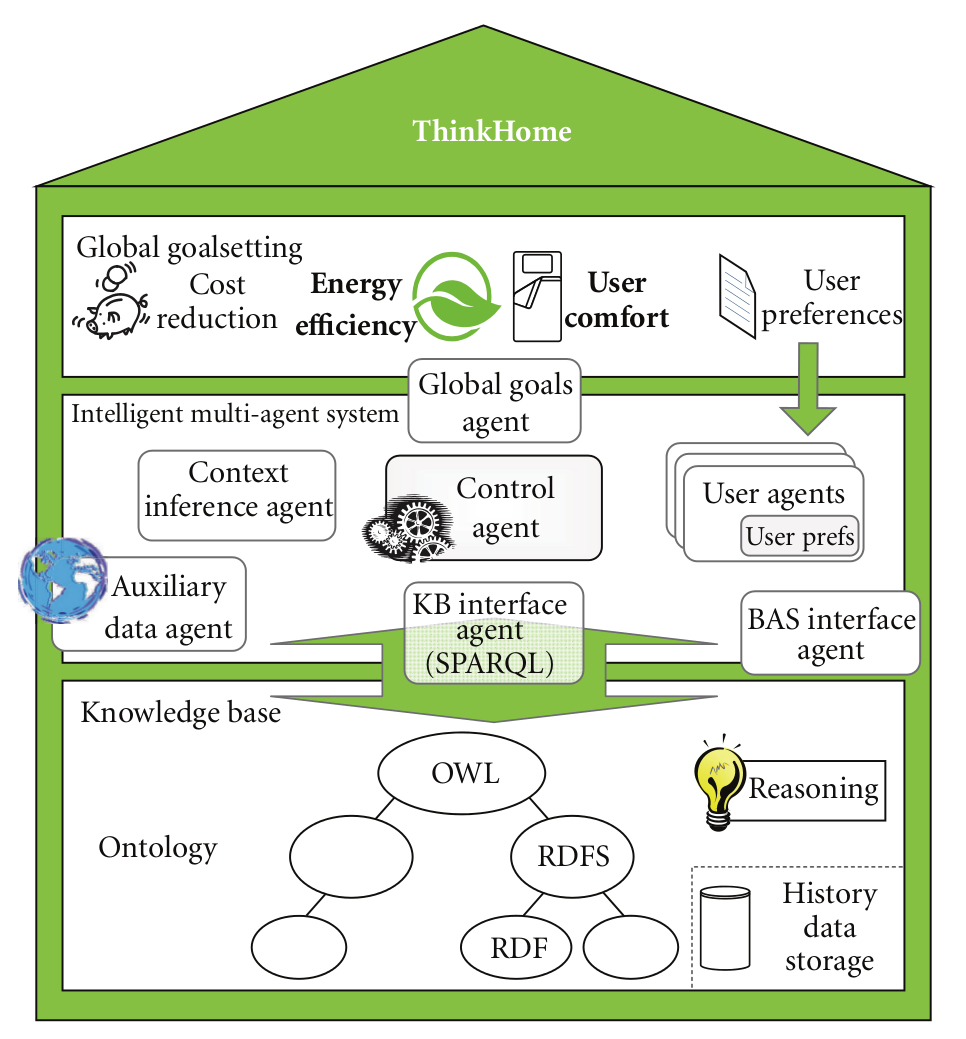
\includegraphics[height=6.5cm]{figures/thinkhome}
	\end{center}
\end{frame}

\section{Existing work}

\subsection{Ontologies}

\begin{frame}{Weather ontologies}
	Several ontologies cover weather data:
	\begin{itemize}
		\item Semantic Sensor Web
		\item SSN Ontology
		\item SWEET
		\item NNEW
		\item …
	\end{itemize}

	Unfortunately, none of them was found to be suitable for smart homes.
\end{frame}

\begin{frame}{OWL-Time}
\end{frame}

\begin{frame}{Basic WGS84 (lat/lon) Vocabulary}
\end{frame}

\begin{frame}{Units of Measurement}
\end{frame}

\subsection{Weather data}

\begin{frame}{Sensors and services}
\end{frame}

\begin{frame}{Weather sensors}
\end{frame}

\begin{frame}{Weather services}
\end{frame}

\begin{frame}{Weather elements}
\end{frame}

\subsection{Ontology design methodologies}

\begin{frame}{Methodologies}
\end{frame}

\begin{frame}{METHONTOLOGY}
\end{frame}

\section{Results}

\subsection{SmartHomeWeather}

\begin{frame}{Competency questions}
\end{frame}

\begin{frame}{Overview}
\end{frame}

\begin{frame}{Concept hierarchies: Weather phenomenon}
\end{frame}

\begin{frame}{Concept hierarchies: Weather state}
\end{frame}

\begin{frame}{Concept hierarchies: Weather report}
\end{frame}

\subsection{Weather Importer}

\begin{frame}{Weather Importer}
\end{frame}

\begin{frame}{SPARQL and SWRL}
\end{frame}

\subsection{Conclusion}

\begin{frame}{Future work}
\end{frame}

\begin{frame}{The end}
\end{frame}

\end{document}


